%!TEX root = doc.tex
\section{Related Work} % (fold)
\label{sec:related_work}

%% Intro to the related work
Some works \cite{garcia2011misia,gormer2011jrep,YooG08,warden2010towards} have approached the problem of complementing Repast and JADE's features by using them together.
We chose to briefly describe two such approaches: MISIA and JRep. They propose combining Repast and \gls{JADE}, allowing the creation of Repast simulations that also take advantage of JADE's networking capabilities and use of \gls{FIPA} standards.

%% MISIA
\subsection{MISIA}
MISIA's approach, as suggested by Figure \ref{fig:misia}, is to use a middle layer that acts as the bridge between two other layers that interact with JADE and Repast Simphony.
By extending the agents in Repast and JADE, communicating through a coordinator and synchronizing their state, these agents work as a single one.

\begin{figure}
	\centering
	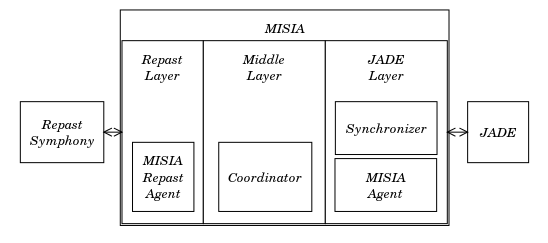
\includegraphics[width=3.0in]{figures/MISIA.pdf}
	\caption{High-level representation of MISIA's architecture (adapted from \cite{garcia2011misia})}
	\label{fig:misia}
\end{figure}

One of the challenges identified by the authors when re-implementing the FIPA interaction protocols was synchronizing them with the Repast tick-based simulation model.
Given JADE's event-driven architecture, MISIA proposes the use of a coordinator agent that informs the JADE-Agent when a tick has passed.
It also proposes its own implementation of the interaction protocols supported by JADE, making them tick-friendly.

%% JREP
\subsection{JRep}
JReps's approach is not as complex as MISIA's.
By having the Repast Simphony agent encapsulate a JADE agent representation, synchronization is immediate and is assured without requiring an external coordinator.
The two agent representations take care of synchronizing any state changes.
Figure \ref{fig:jrep} represents the basic structure of JRep.

\begin{figure}
	\centering
	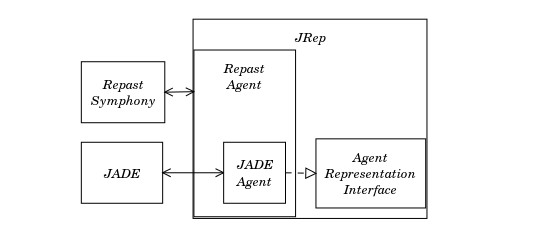
\includegraphics[width=2.1in]{figures/jrep.pdf}
	\caption{High-level representation of JRep's architecture}
	\label{fig:jrep}
\end{figure}

Each agent takes care of interfacing their respective frameworks. The interaction between agents in JRep is performed using FIPA ACL and the protocol implementations are those provided by the JADE platform. Similarly to MISIA, an Agent Representation Interface is used to introduce the concept of schedule in the JADE agent


%% COMPARISON
\subsection{Comparison with \apiname{}}

JADE is a very rich platform but, for many simulation scenarios, the overhead introduced by it has a significant impact on simulation performance \cite{mengistu2008scalability}. \apiname{}, as we describe with more detail in Section \ref{sec:proposal}, uses an architecture that is conceptually very close to JADE's but tailored for Repast with no extra dependencies. Moreover, the API could be used with other simulation frameworks with little adaptation.

As suggested by Figure \ref{fig:related-repacl}, \apiname{}'s general structure is simpler than that of JRep and MISIA. Our API does not intend to maintain an active connection to a JADE platform, eliminating the need for synchronization. Instead, our goal is to replicate in our API the main features of JADE, allowing for a straightforward and dependency free feature mapping between our API and JADE.

\begin{figure}
	\centering
	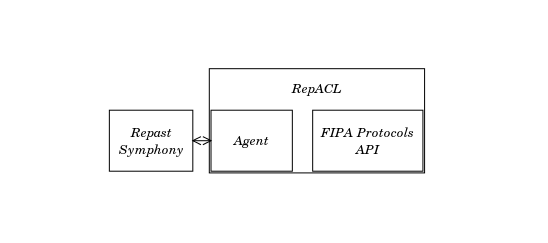
\includegraphics[width=2.1in]{figures/repacl.pdf}
	\caption{Basic structure of \apiname{}}
	\label{fig:related-repacl}
\end{figure}

In both MISIA and JRep, even though they attempt to integrate the features from both JADE and Repast, as far as Repast simulations are concerned JADE's multi-threaded infrastructure affects their performance very significantly. The main advantage of our approach is, therefore, the possibility of using Repast with JADE features, namely FIPA specifications including interaction protocols, without the need to interface with JADE. In Section \ref{sec:proposal} we provide a more detailed description of \apiname{}.

